\documentclass[10pt,twocolumn,letterpaper]{article}
\usepackage{cvpr}
\usepackage[hyphens]{url}
\usepackage{times}
\usepackage{graphicx}
\usepackage{amsmath}
\usepackage{amssymb}
\usepackage[pagebackref=true,breaklinks=true,colorlinks,bookmarks=false]{hyperref}
\def\GroupID{G01} % <------- ENTER YOUR COMP 6321 group number here
\setlength{\parindent}{2em}
\setlength{\parskip}{0em}
\renewcommand{\baselinestretch}{1}

\begin{document}
\title{Is it Fake News? A Comparison of Traditional Machine Learning Models and Deep Learning Models for News Article Classification}
\author{Giselle Martel ID: 26352936 \and Firas Sawan ID: 26487815}
\maketitle
\begin{abstract}
\small
"Fake news" is a term which we hear more often in contemporary times, and "is part of a larger spectrum ranging from unintentional misinformation (e.g., sloppy reporting) to intentional disinformation (e.g., propaganda)"\cite{doi:https://doi.org/10.1002/9781118841570.iejs0128}. The spread of falsehoods and inaccuracies through social media and online news sources undermines societal progress, and can spawn a multitude of negative effects [CITATION NEEDED]. Thus, the objective of our project is explore the feasibility and performance of existing supervised machine learning and natural language processing techniques in the identification of "fake news" to explore solutions that address misinformation in the digital age. We compare binary classification performance of news articles into "fake" or "real" categories by training six different machine learning models. Traditional classifiers such as Logistic Regression, Decision Tree, Random Forest, Support Vector Machines, and Multinomial Naive Bayes classification were utilized in our experiments, in addition to a Convolutional Neural Network. The results show that Logistic regression has the highest level of accuracy and lowest level of overfitting, thus it was generally the best model to use for classifying articles into the two categories. This classifier was followed in terms of accuracy and performance by the other 4 classifiers in the order mentioned above and the results are presented in the following report. 
\end{abstract} 

%------------------------------------------------------------------------
\section{Introduction}
\small
The term “fake news” mainly refers to false or inaccurate information that is mistakenly or inadvertently created or spread. Such information is often presented in the form of reputable news, despite the often omission of verifiable facts or sources, deliberately inflammatory language, and the presentation of an issue from one polarized viewpoint [CITATION NEEDED]. In regards to the current COVID-19 global health crisis we are facing, and the recent 2020 U.S. elections, we have witnessed as a society the exponential spread of conspiracies, accusations, and falsehoods which is often fueled by misleading or suspicious sources [CITATION NEEDED]. Such a situation can have a multitude of negative outcomes and undermines progress in several areas of society ranging from politics, health, economics, social justice, and beyond [CITATION NEEDED].\par

Given our concern with this issue, the purpose of our project is to explore machine learning models that can aid in the identification of misleading or untruthful news articles online. We would like to identify, if any, existing popular machine learning models that could accurately classify online new sources by text into "fake" and "real" labels. We will compare the the pros and cons of five different traditional supervised models in text classification; which include Logistic Regression, Decision Tree, Random Forest, Support Vector Machine, and Multinomial Naive Bayes classifiers. In addition, we will compare the results with a supervised deep Convolutional Neural Network. Hyper-parameter tuning will be employed for all models in an attempt to generate a successful result.\par

To train our collection of models, we utilized an existing dataset from Kaggle of news articles collected between 2015-2018 [CITATION NEEDED], in addition to data which was collected via scraping of more recent articles from both trusted and illegitimate news sources. The following scraped sources were included and labelled as "real" news: CBC news, CTV news, Global news, The Guardian, Fox News, NBC, The Washington Post, BBC, and CNN which are all generally recognized as reputable. More questionable scraped sources such as Breitbart, Infowars, Prntly, National Report, and Daily Buzz Live were labelled as "fake" and included in the dataset. In addition, well-know satirical news sources such as "The Onion" and "The Beaverton" were also included in the data and labelled as "fake". The figure below depicts the structure of the dataset from Kaggle, and the following figure depicts the raw structure of the scraped data before preprocessing:
\begin{center}
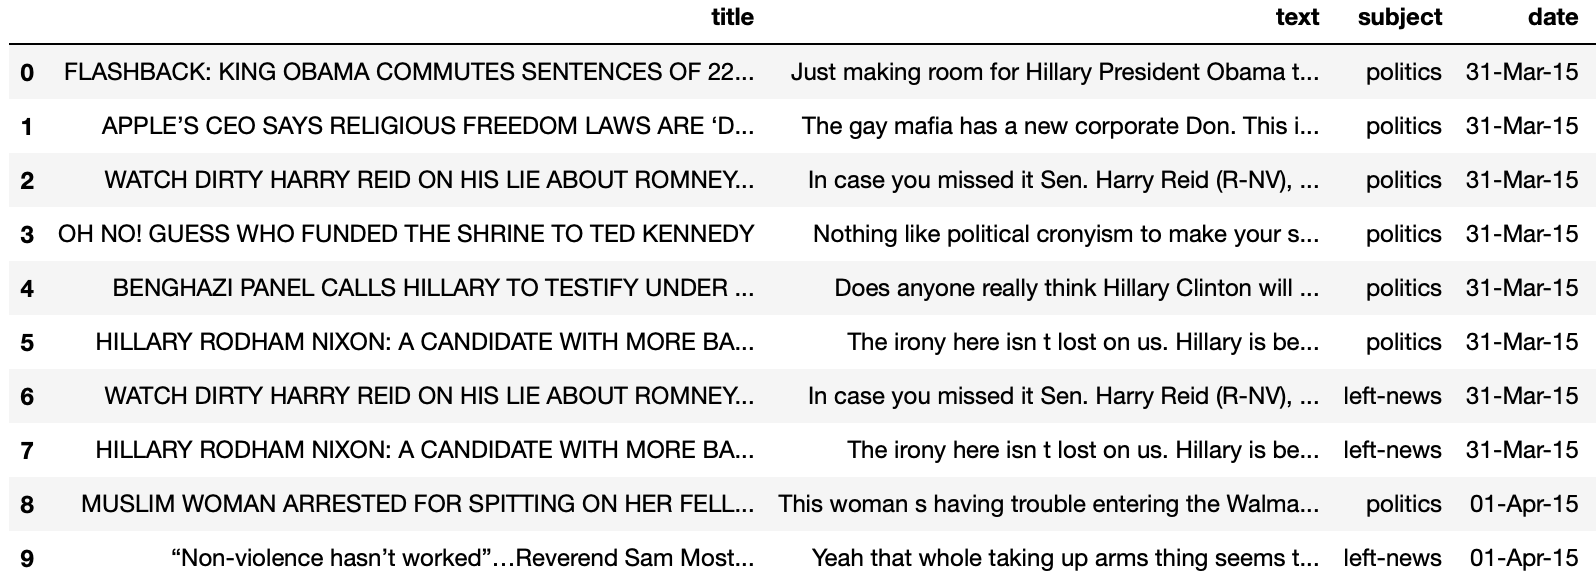
\includegraphics[scale=0.3]{dt_example.png}
\end{center}
\begin{center}
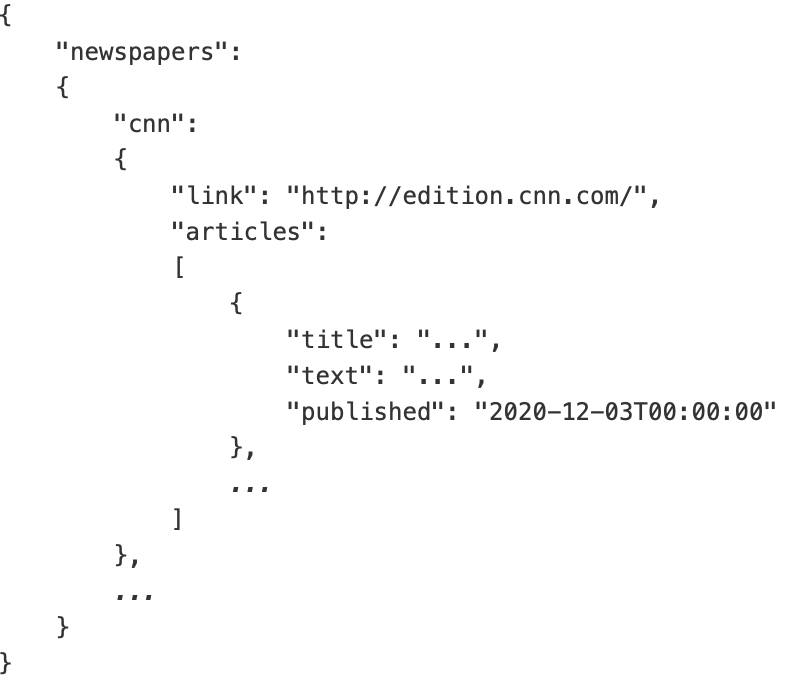
\includegraphics[scale=0.3]{scraped_example.png}
\end{center}
Our inspiration to utilize the Kaggle dataset in addition to a scraping approach came from a similar experiment in news classification conducted by Ria Gandhi [CITATION HERE]. In addition, her approach in preprocessing of the data and her model selection were somewhat replicated in our project, albeit with many changes to implementation details and parameter tuning. The underlying goal of this experiment is to present the respective results from each model and compare their overall performance in classification. The results of our model training and the generated predictions will be presented analyzed in this report. Detailed graphs, confusion matrices, metrics measurement, and other results  for each of the classifiers as well as a report of accuracy, precision and recall metrics. 


%------------------------------------------------------------------------
\section{Methodology \& Experimental Results}
\small
The first step in our experiment was to carry out the preprocessing of the raw dataset. Preprocessing included steps such as the cleanup of the raw data from both Kaggle and scraped sources into the desired format, and then removing empty data cells, punctuation from each article's text formatting, and applying tokenization to each entry in the dataset using the Natural Language Processing Toolkit library. Tokenization allows for the extraction of all unique words from each article into a list of words as opposed to a single string object, while providing the option to exclude stop-words for words that are overtly present in the data or for words that the model should be agnostic to. Additionally in this process a dictionary of all the words in the dataset (i.e. vocabulary) was generated to define all the training features. For the purposes of this project, we chose to omit common words of the English language in addition to certain words that appear on every entry of the Kaggle dataset, notably "Reuters", since each "real" entry contained a reference to this well-known reputable news source.  In addition, we also applied a lemmatization to group together words that appear in several (inflected) forms. For instance, words that imply the same meaning such as "lying" and "lie" may be grouped together during this process.\par

After data cleanup and text tokenization, we vectorized the article entries by applying a TF-IDF Vectorizer to assign a normalized feature frequency mapping to our list of tokenized articles, which returns a sparse matrix that can be utilized for training all of the traditional machine learning models. The Convolutional Neural Network conversely was trained using a Count Vectorizer, which uses a non-normalized form of the frequency mapping (i.e. integer form instead of normalized floats) since this model classifies based on frequencies. This appeared to generate more desirable result for the Convolutional Neural Network during training and evaluation. After tokenization and generating the features to train the model with, the next step is to include the corresponding label for each article in the data, with the choice being "real" or "fake" and then combine all entries into a data frame. The last step of preprocessing was to split the data into testing and training samples, with a 30\% and 70\% split respectively.\par

The first model that was trained on the preprocessed data was the Logistic Regression classifier. We opted to tune the inverse regularization hyperparameter with 13 values in the logarithmic space ranging from 10\textsuperscript{-6} to 10\textsuperscript{6}. Hyperparameter tuning on this estimator was carried out by using the GridSearchCV method to determine the inverse regularization value that generated the best cross-validation core, which happened to be C=10. Choosing the optimal inverse regularization parameter yields a result with the most ideal trade-off between overfitting and accuracy.  In addition, we also calculated the training and testing accuracy for each hyperparameter, and plotted the result (as shown in the figure below). The small margin of difference between the test and training scores in the graph generally indicates that the Logistic Regression model has little overfitting, and that the test and training scores tend to converge which are both desirable outcomes.\par

After determining the best hyperparameter and training the model, the testing features were fed into the model to obtain a prediction of the corresponding labels, where "real" news is encoded as 0 and "fake" news is encoded as 1. We subsequently generated a graph of each of the training and testing scores as well as a confusion matrix (Figure~\ref{first_figure}) that helped us visualize predictions of the new articles. Please refer to the appendix to view side-by-side comparison of the distribution of fake vs. real news (Figure~\ref{piechart_1}). The model achieved a testing accuracy of 91.34\%, a mean squared error of 9.62\% and a precision of 90.78\% with a very low overfitting value of 0.009. \\

\begin{figure}[h]
   \begin{center}
        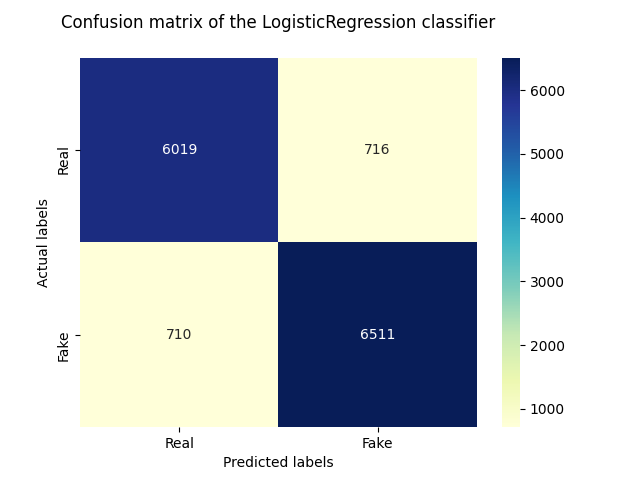
\includegraphics[width=\linewidth]{graphs/LR/confusion_matrix.png}
        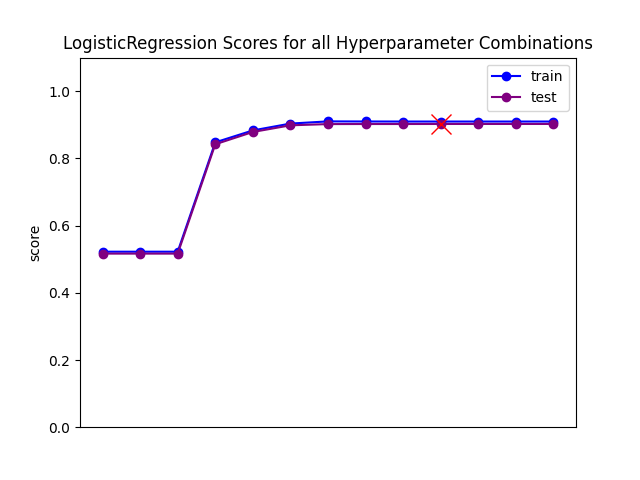
\includegraphics[width=\linewidth]{graphs/LR/scores_plot.png}
   \end{center}
        \vspace*{-5mm}
        \caption{\label{first_figure}}
\end{figure}
The Decision Tree classifier was the next model trained in the experiment. This model predicts the correct label for a particular article by learning simple decision rules inferred from the training data features. Only the max depth hyperparameter was used to train the model, whose value was likewise determined via cross-validation. The hyperparameter search was carried out with 50 values in the linear space ranging from 2 to 100. It was important to choose a wide enough range to ensure a better estimator, but without compromising computational performance which is the case with larger tree depths. The grid search yielded an optimal maximum tree depth parameter of 16. The model's overfitting value was also calculated based on the training and held-out scores over each hyperparameter, and similarly the result was graphed like with the Logistic Regression model. The result of the predictions performed by the Decision Tree classifier are depicted in the confusion matrix in Figure~\ref{Second_figure} in the appendix. The model achieved an accuracy of 86.14\%, a mean squared error of 13.86\% and a precision of 86.12\% with an overfitting value of 1.096.\par

The Random Forest classifier fits a number of Decision Tree classifiers on various sub-samples of a dataset, and generally yields better results than a single Decision Tree since it takes advantage of averaging. Predictive accuracy can be improved while also controlling over-fitting to a satisfying degree. Just like with the previous 2 models, a hyperparameter search using GridSearchCV was conducted to find the optimal maximum depth and number of estimators. The chosen parameters for the search were values in the linear space between 2 and 14 for max depth, and 10 values in the linear space between 2 and 20. It was important to perform the hyperparameter search in a reasonable range, in order to avoid excessively expensive computations and infeasible training situations given the time constraints of our experiment and size of our dataset. The hyperparameter search yielded the optimal tree depth as 14 and the optimal number of classifiers (decision trees) as 20. As with the previous models, a plot of the training and held-out scores and the prediction confusion matrix is depicted below, in addition to a plot displaying the feature importances for the top 25 words in Figure~\ref{Third_figure} in the appendix. Figure~\ref{piechart_3} shows the distribution of labels for the true and predicted. The model achieved an accuracy of 91.11\%, a mean squared error of 8.89\% and a precision of 91.25\% with an overfitting value of 1.42.\par

A Support Vector Machine model, which is a form of supervised learning, was then used to further help us in our quest for category prediction and classification. This model had an advantage of being memory efficient in the sense that it uses a subset of training points in the decision function called support vectors. In terms of the parameters used, we performed a hyperparameter search over 2 types of kernels, namely a Gaussian kernel of type 'rbf' and a linear kernel, with 5 values of C and gamma both ranging within the logarithmic space from 10\textsuperscript{-2} to 10\textsuperscript{2}. The best estimator with kernel='rbf', C=0.01, and gamma = 0.179 was returned by the grid search, and thus used in the predictions on the testing set. Refer to Figure~\ref{fourth_figure} in the appendix to visualize the result. The model achieved an accuracy of 60.73\%, a mean squared error of 39.27\% and a precision of 57.89\%.\par
Multinomial Naive Bayesian classifier was the next model chosen given its suitability for classification of discrete feature, such as the tokenized text in our preprocessed dataset. Like with the previous models, a grid search was performed over the hyperparameters alpha (discrete values between 0 and 50) and fit\_prior (true or false) to obtain the ideal estimator. The best estimator with fit\_prior=true and alpha=1.585 was returned by the grid search, and thus used in the predictions on the testing set. Refer to Figure~\ref{fifth_figure}. The model achieved an accuracy of 87.408\%, a mean squared error of 12.59\% and a precision of 90.01\% with an overfitting value of 0.022. \par

The last part of our experiment was to compare the classification of a supervised deep-learning model in contrast to more traditional machine learning models. We opted to use a Convolutional Neural Network, since it is well suited for text classification based on the frequency of occurrence for words. Since our preprocessing takes the frequencies of each into account, we felt that this model would be best suited to our data's structure. The implementation of this model relied heavily on the tutorial of Deep Learning Engineer Fernando Lopez [CITATION NEEDED]. In terms of training parameters, we first opted to use a batch size of 108, 24 epochs, and a learning rate of 0.001. The losses generated during training and evaluation were diverging, since the learning rate was too large for the gradient descent, and was overshooting at each epoch. After tuning the learning rate to be a smaller value of 0.0001, the result was much better, with a solution that was converging with each epoch. Refer to the Figure~\ref{sixth_figure} below to visualize the results. In the appendix, plots depicting the accuracies over each epoch are shown Figure~\ref{seventh_figure}.
\begin{figure}[h]
   \begin{center}
       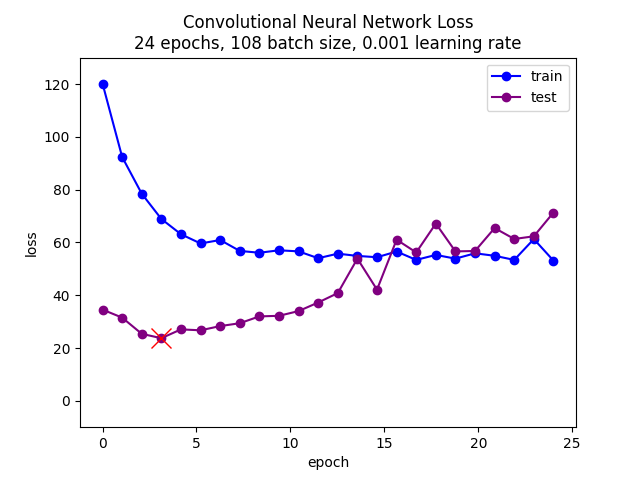
\includegraphics[width=\linewidth]{graphs/CNN/higher_learning_rate_loss_plot.png}
        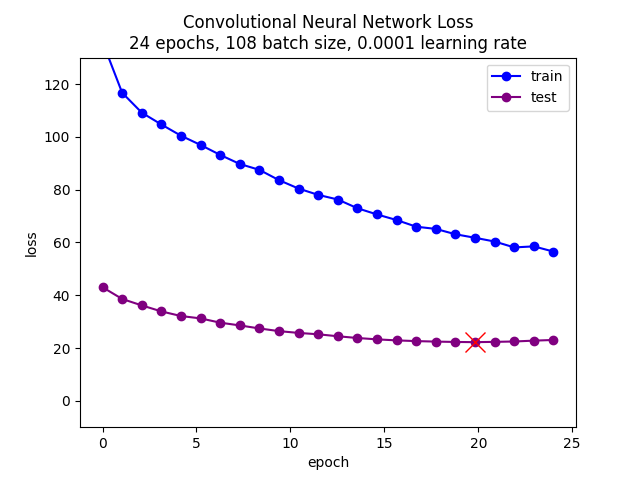
\includegraphics[width=\linewidth]{graphs/CNN/loss_plot.png}
   \end{center}
        \vspace*{-6mm}
        \caption{\label{sixth_figure}}
\end{figure}

%------------------------------------------------------------------------
\section{Conclusions}
\small
As discussed in the previous section our quest for article classification involved training various types of classifiers each taking their own set of parameters to achieve the most ideal results possible. We notice that logistic regression had the highest accuracy at 91.34\% when it came to correctly classifying our tokenized data into the Fake and Real categories. The confusion matrix generated for this model shows that it correctly classified 6014 words into the "Real" category and 6618 words into the "Fake" category and overfitting. The degree of overfitting for this classifier was also the lowest obtained at 0.009. This allows us to conclude that logistic regression classifier was the best model to use on our preprocessed data. \par

Logistic regression was closely followed by the Random forest classifier with a classification accuracy of 91.11\%. The confusion matrix generated for this classifier shows very similar results to that of the logistic regression with 6060 articles correctly classified into the "Real" category and 6675 articles into the "Fake" category. The model, however, had a much higher overfitting value at 1.421. This means that although the classifiers were very close in terms of their accuracy, logistic regression remains at an advantage given that it had much less overfitting of data. \par

The Multinomial Naive Bayesian model comes in third place in terms of performance with a classification accuracy of 87.41\%. Its confusion matrix shows that the model was able to successfully classify 6011 articles into the "Real" category and 6206 articles into the "Fake" category. The model has an advantage over the other two that it was the fastest to run and classify the data with a very low degree of overfitting at 0.022. In total the model took approximately 4 seconds to run from start to finish including the hyper parameter search that occupies the bulk of execution time. Perhaps this model would be a better fit to use compared to the logistic regression classifier if the goal is to achieve speed over accuracy. \par

Decision Tree Classifier follows the Bayesian model closely with a classification accuracy of 86.14\%. Its confusion matrix shows that the mode was able to correctly classify 5674 articles into the "Real" category and 6366 articles into the "Fake" category. The model was significantly slower to run than the Bayesian model at 1.2 minutes vs the 3 seconds the Bayesian model took to classify our data. It also had a much higher overfitting value at 1.096 and thus we can conclude that the Naive Bayesian model is better employed to solve our particular problem on the provided dataset.  \par

The support vector machine classifier was the slowest to run out of all classifiers taking approximately 10.8 minutes to fully classify the data. It had the lowest classification accuracy of 60.73\% compared to other models and an overfitting value of 0.142. The model was successfully able to classify 1929 articles into the "Real" category compared and 6559 into the "Fake" category. This information allows us to conclude that although the overfitting value for the model was relatively low, that advantage is outweighed by the slow run time for the model and a logistic regression model can achieve better results at a faster pace and with significantly less overfitting. \par

Finally the CNN.... \par

Overall, we can conclude generally machine learning models can classify fake and real news with a relatively high degree of accuracy. It is important to note that every step of the process was important. Correctly cleaning the raw data, tokenizing it with wisely chosen stopwords, using lemmatization, and applying the correct vectorizer depending on the model all have contributed to the higher rates of accuracy. The least performant of the classifier, the SVM, was the only model that appeared to diverge and had a high mean squared error. This is likely indicative of poorly chose hyperparameters. It would be a good idea to try a different set of hyperparameters for the cross-validation in order to yield a more ideal result. 
Please refer to the appendix to see more graphs depicting the classification results.


{\small
\raggedright
\bibliographystyle{ieeetr}
\bibliography{bibliography}
}

\newpage
\appendix
\onecolumn
%-------------------------------------------------------------------------
\section*{Appendix: Extra Results}\centering
\begin{table*}[!hb]\centering
   \begin{center}
   \begin{tabular}{|l|c|c|c|c|c|}
   \hline
    Classifier & Accuracy & Mean Squared Error & Precision & Recall & fscore\\
   \hline\hline
   Naive Bayes & 92.33\% & 27.7\% & 94.25\% & 90.87\% & 92.53\% \\
   Decision Tree & 99.22\% & 8.79\% & 99.03\% & 99.48\% & 99.26\% \\
   Random forest & 94.40\% & 23.60\% & 93.99\% & 95.41\% & 94.69\%\\
   Support Vector Machine & 90.90\% & 30.04\% & 91.24\% & 91.51\% & 91.38\% \\
   Logistic Regression & 99.08\% & 9.55\% & 99.14\% & 99.10\% & 99.13\% \\
   \hline
   \end{tabular}
   \end{center}
   \caption{Summary of Traditional ML Model Results\label{first_table}}
\end{table*}

\begin{figure}[h]
   \begin{center}
        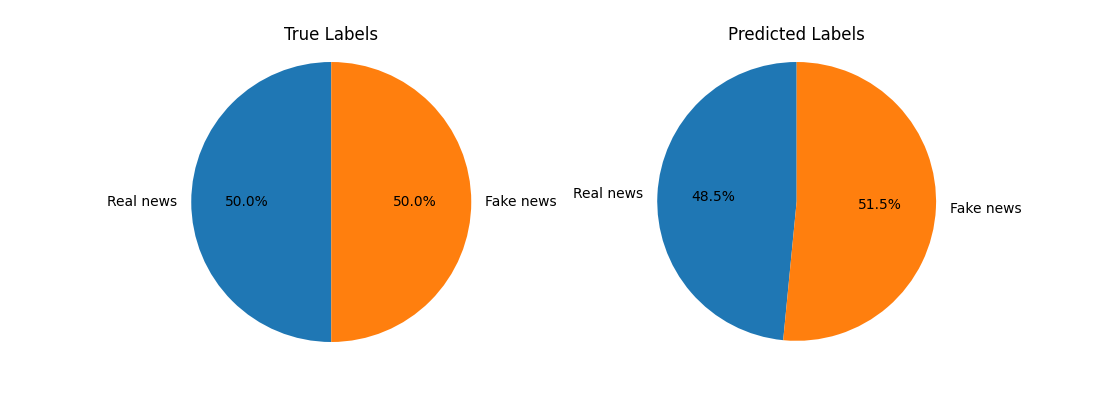
\includegraphics[scale=0.6]{graphs/LR/piechart.png}
   \end{center}
\vspace*{-5mm}
\caption{Logistic Regression results \label{piechart_1}}
\end{figure}

\begin{figure}[h]
   \begin{center}
        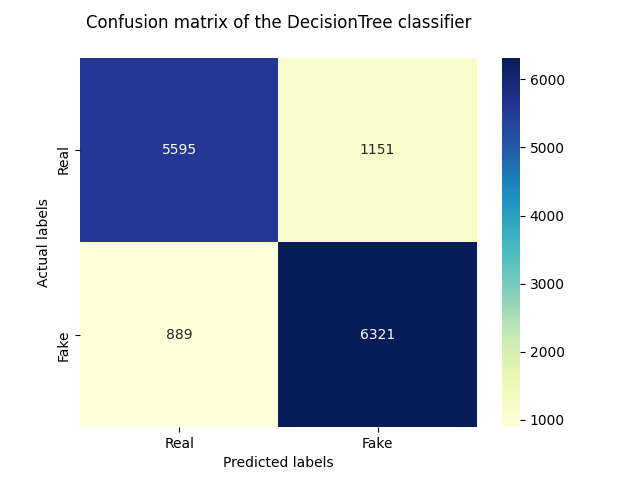
\includegraphics[scale=0.8]{graphs/DT/confusion_matrix.png}
        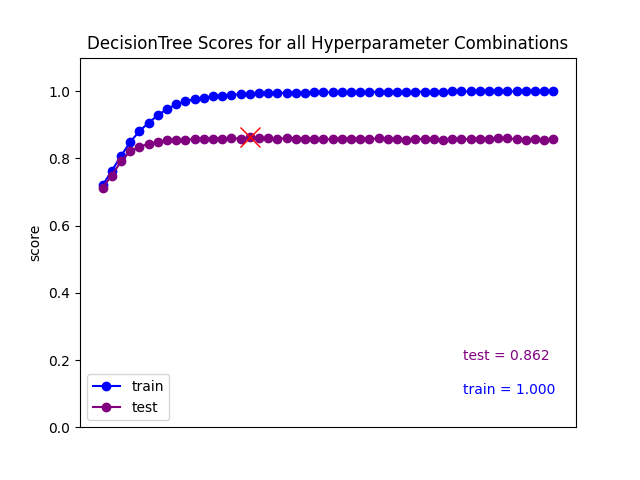
\includegraphics[scale=0.8]{graphs/DT/scores_plot.png}
        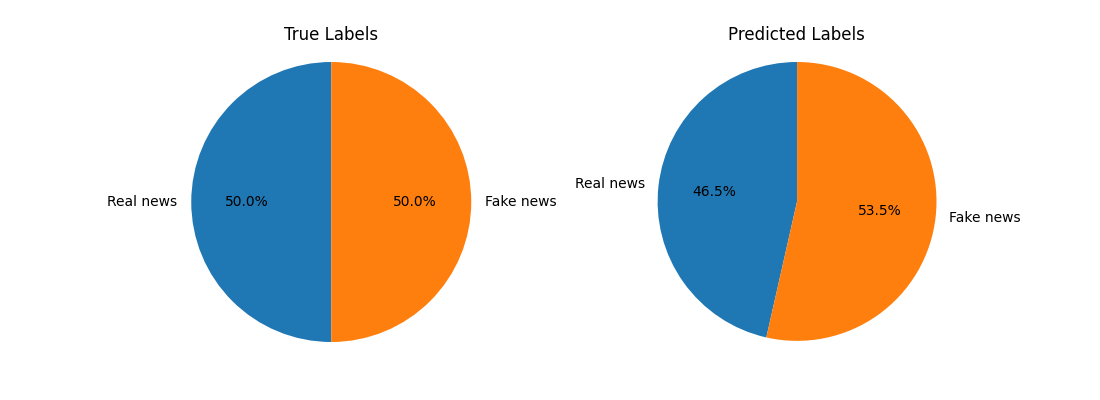
\includegraphics[scale=0.6]{graphs/DT/piechart.png}
   \end{center}
        \vspace*{-5mm}
        \caption{\label{Second_figure}}
\end{figure}


\begin{figure}[h]
   \begin{center}
        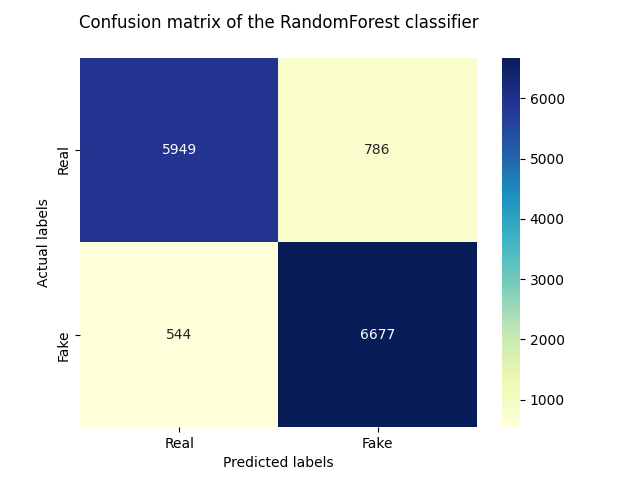
\includegraphics[scale=0.6]{graphs/RF/confusion_matrix.png}
        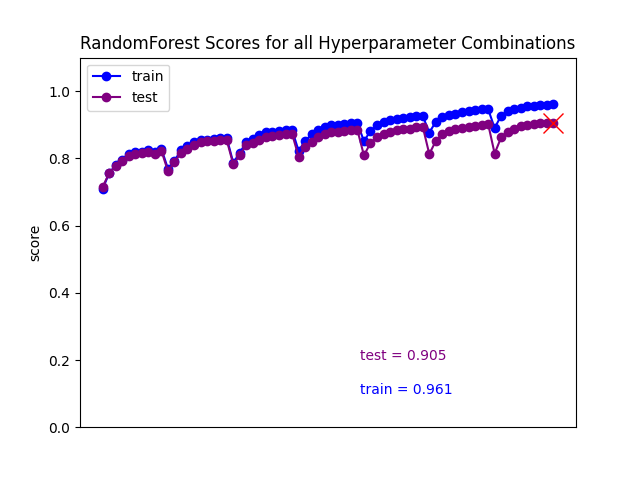
\includegraphics[scale=0.6]{graphs/RF/scores_plot.png}
        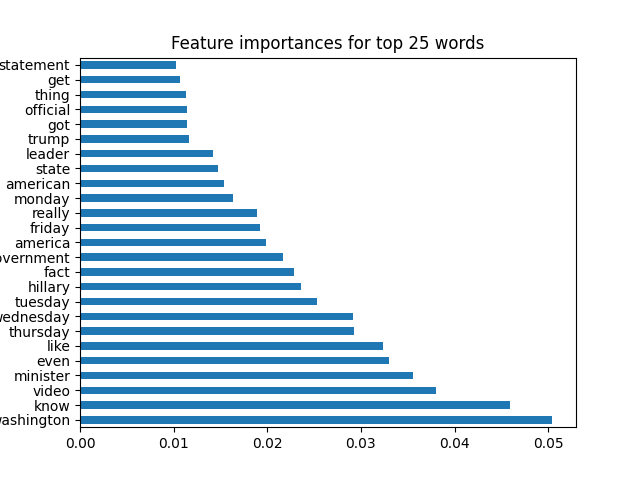
\includegraphics[scale=0.6]{graphs/RF/feature_importances.png}
   \end{center}
        \vspace*{-5mm}
        \caption{\label{Third_figure}}
\end{figure}

\begin{figure}[h]
   \begin{center}
        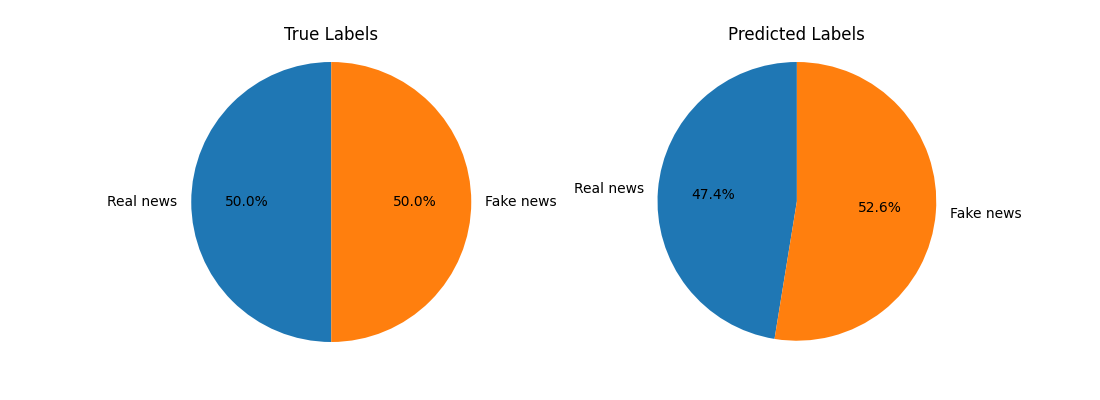
\includegraphics[scale=0.6]{graphs/RF/piechart.png}
   \end{center}
\vspace*{-5mm}
\caption{Random Forest results \label{piechart_3}}
\end{figure}

\begin{figure}[h]
   \begin{center}
        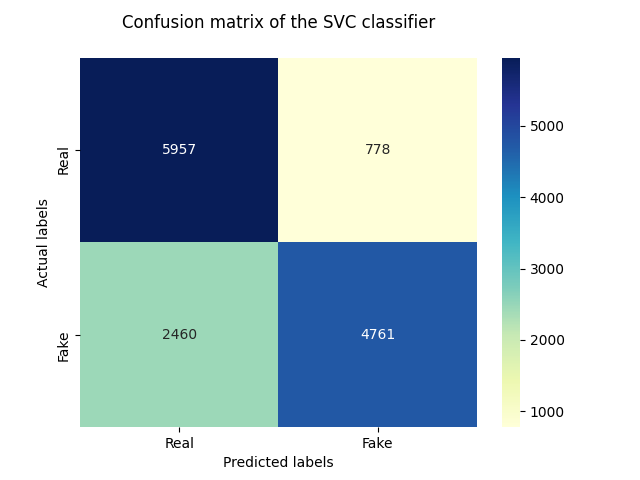
\includegraphics[scale=0.6]{graphs/SVC/confusion_matrix.png}
        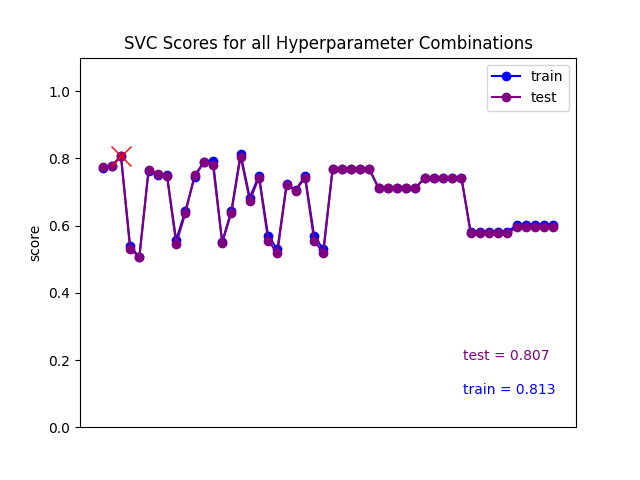
\includegraphics[scale=0.6]{graphs/SVC/scores_plot.png}
        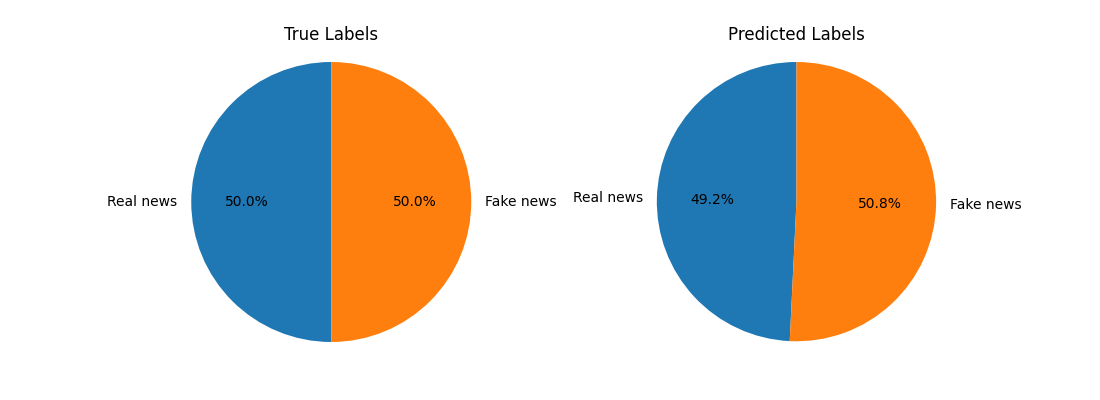
\includegraphics[scale=0.6]{graphs/SVC/piechart.png}
   \end{center}
        \vspace*{-5mm}
        \caption{\label{fourth_figure}}
\end{figure}

\begin{figure}[h]
   \begin{center}
        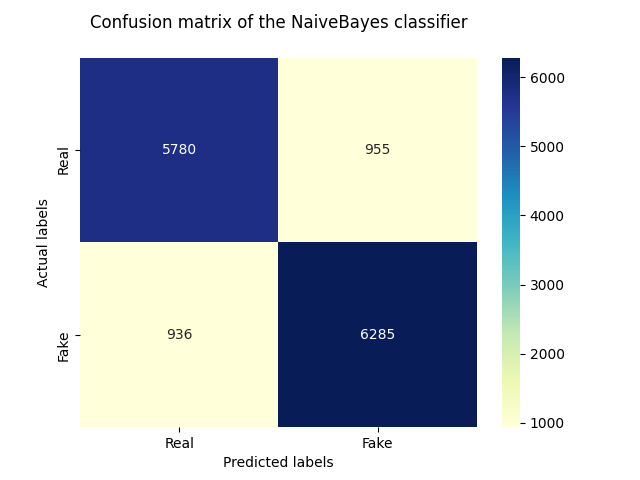
\includegraphics[scale=0.6]{graphs/NB/confusion_matrix.png}
        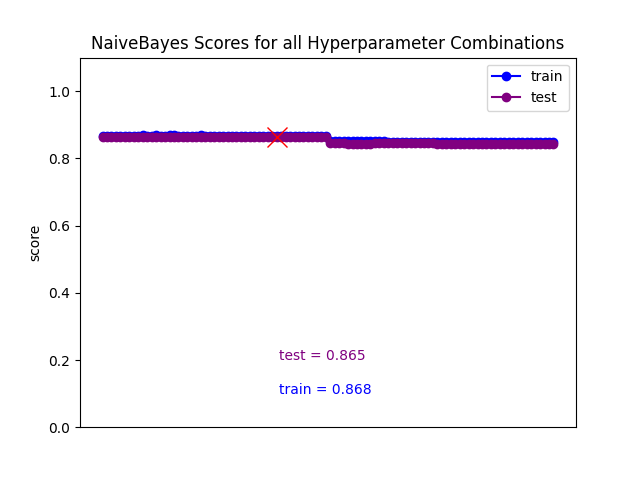
\includegraphics[scale=0.6]{graphs/NB/scores_plot.png}
        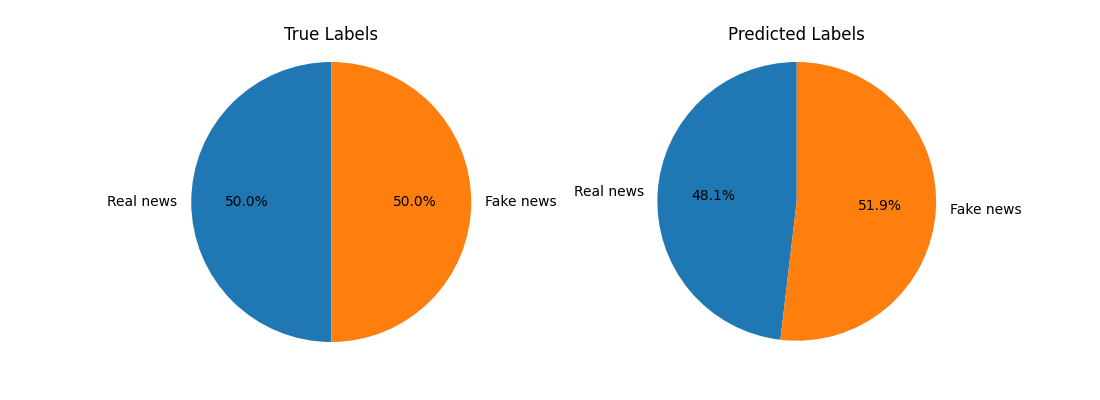
\includegraphics[scale=0.6]{graphs/NB/piechart.png}
   \end{center}
        \vspace*{-5mm}
        \caption{\label{fifth_figure}}
\end{figure}

\begin{figure}[h]
   \begin{center}
       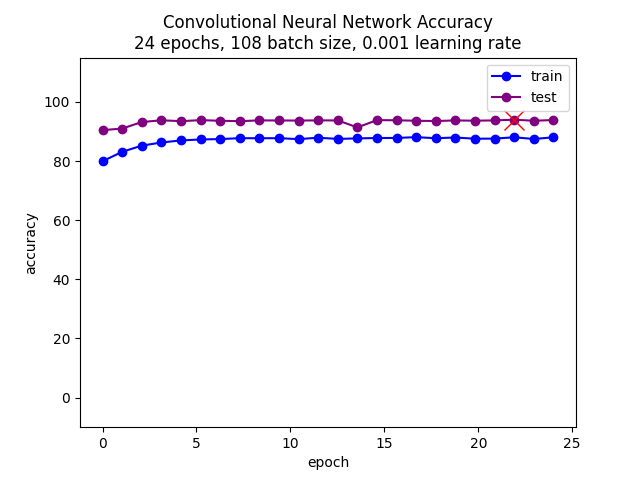
\includegraphics[scale=0.8]{graphs/CNN/higher_learning_rate_accuracies_plot.png}
        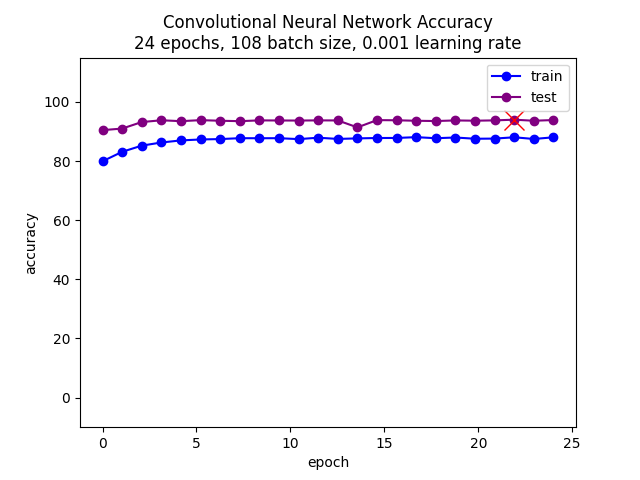
\includegraphics[scale=0.8]{graphs/CNN/accuracies_plot.png}
   \end{center}
        \vspace*{-5mm}
        \caption{\label{seventh_figure}}
\end{figure}

\end{document}
